\documentclass[10pt,twocolumn,letterpaper]{article}

\usepackage{cvpr}
\usepackage{times}
\usepackage{epsfig}
\usepackage{graphicx}
\usepackage{amsmath}
\usepackage{amssymb}
% Include other packages here, before hyperref.
% \usepackage[outdir=./]{epstopdf}

% If you comment hyperref and then uncomment it, you should delete
% egpaper.aux before re-running latex.  (Or just hit 'q' on the first latex
% run, let it finish, and you should be clear).
\usepackage[breaklinks=true,bookmarks=false]{hyperref}

% \cvprfinalcopy % *** Uncomment this line for the final submission

\def\cvprPaperID{3510} % *** Enter the CVPR Paper ID here
\def\httilde{\mbox{\tt\raisebox{-.5ex}{\symbol{126}}}}

%% Custom control sequences
\let\oldPr\Pr
\newcommand{\bR}{\mathbb{R}}
\renewcommand*{\Pr}[1]{\mathbb{P}\left( #1 \right)}
\newcommand{\mat}[1]{\mathbf{#1}}
\DeclareMathOperator*{\argmax}{arg\,max}
\DeclareMathOperator*{\argmin}{arg\,min}
\newcommand{\tr}{\mathbf{tr}}
\newcommand{\cross}[1]{[#1]_{\times}}


% Pages are numbered in submission mode, and unnumbered in camera-ready
%\ifcvprfinal\pagestyle{empty}\fi
\setcounter{page}{1}
\begin{document}

%%%%%%%%% TITLE
% \title{All Graphs Lead to Rome: \\
% Cycle Consistent Multi-View Representations Using Graph CNNs}
\title{All Graphs Lead to Rome: Learning Geometric and Cycle Consistent Representations with Graph CNNs}

\author{Stephen Phillips, Kostas Daniilidis \\
GRASP Labratory, University of Pennsylvania\\
{\tt\small \{stephi, kostas\}@seas.upenn.edu}
% For a paper whose authors are all at the same institution,
% omit the following lines up until the closing ``}''.
% Additional authors and addresses can be added with ``\and'',
% just like the second author.
% To save space, use either the email address or home page, not both
% \and
% Second Author\\
% Institution2\\
% First line of institution2 address\\
% {\tt\small secondauthor@i2.org}
}

% When placing figures in \LaTeX, it's almost always best to use
% \verb+\includegraphics+, and to specify the  figure width as a multiple of
% the line width as in the example below
% {\small\begin{verbatim}
%    \usepackage[dvips]{graphicx} ...
%    \includegraphics[width=0.8\linewidth]
%                    {myfile.eps}
% \end{verbatim}
% }


\maketitle
%\thispagestyle{empty}

% Papers, excluding the references section,
% must be no longer than eight pages in length. The references section

%%%%%%%%% ABSTRACT
% We present a learning technique for refining multi-image feature matches in an unsupervised fashion.
\begin{abstract}
    Image feature matching is a fundametal part of many geometric computer vision applications, and using multiple images can improve performance.
    In this work, we formulate the multi-image matching problem as a graph embedding problem then use a Graph Neural Network to learn an appropriate embedding function for aligning image features. % How to talk about the universe of features here without going too much into the weeds??
    We use cycle consistency to train our network in an unsupervised fashion since ground truth correspondence is difficult or expensive to come by in many real world datasets.
    In addtion, geometric consistency losses can be added at train time, even if the information is not available in the test set, unlike previous optimization based methods.
    To the best of our knowledge, no other works have used learning for multi-image feature matching.
    Our experiments show that our method is competitive with other optimization based approaches.
\end{abstract}

%%%%%%%%% BODY TEXT
\section{Introduction}

Feature matching is an essential part of Structure from Motion and many geometric computer vision applications.
The goal in multi-image feature matching is to take 2D image locations from three or more images and find which ones correspond to the same point in the 3D scene.
Methods such as SIFT feature matching \cite{lowe2004distinctive} and RANSAC \cite{fischler1981random} have been standard for solving this for decades.
However RANSAC-based approaches are limited for matching pairs of images.
Other works, such as Wang et al. \cite{wang2017multi}, have shown improvement in performance by enforcing consistency between multiple images.
% However we still have not fully answered the question: What are the best image features to describe multiple views of the same scene?

Deep learning has revolutionized how image features are computed \cite{yi2016lift}, and so we would like to leverage this to compute better scene features.
Typically when applied to image or feature matching, deep neural networks (DNNs) are trained with photometric losses, directly using pixel color values.
However direct, pixel-based losses have are not robust to the many confounding factors in the environment, such as lighting and view-point changes.
Using features designed to deal with these condfounding factors improves robustness to them, 
and learning may improve robustness even further.

\begin{figure}[t]
\begin{center}
  % \fbox{\rule{0pt}{2in} \rule{0.9\linewidth}{0pt}}
  \includegraphics[width=0.8\linewidth]{figures/CycleConsistencyBasic.pdf}
\end{center}
  \caption{
    Example of multi-image matching, with images from Rome16K dataset \cite{li2010location}.
    In this example, an error in matching leads to an inconsistent cycle (shown in red), ideally these pairwise matches would be consistent.
    We improve consistency between pairwise matches in the multi-view matching problem by training a neural net with cycle consistency.
  }
\label{fig:cycconsistex}
\label{fig:onecol}
\end{figure}

%------------------------------------------------------------------------
\begin{figure*}[t]
\begin{center}
  % \fbox{\rule{0pt}{2in} \rule{0.9\linewidth}{0pt}}
  \includegraphics[width=0.8\linewidth]{figures/CycleConsistencyMainFigure.pdf}
\end{center}
  \caption{
    An outline of the pipeline of this work.
    The Graph Convolutional Neural Network (GCN) \cite{kipf2016semi} takes as input the graph of matches and then outputs a low rank embedding of the adjacency matrix of the graph.
    The GCN operates on an embedding over the nodes of the graph.
    In the figure, the the GCN node embeddings are represented by different colors.
    The final embedding is used to construct a pairwise similarity matrix, which ideally should be a low dimensional cycle consistent representation of the graph adjacency matrix.
    We train the network using a reconstruction loss on the similarity matrix.
    In addition, we can use geometric information at to assist training the network, even if we do not have that geometric information at testing time such as epipolar constraints on the point locations or higher order geometric constraints.
  }
\label{fig:pipeline}
\label{fig:onecol}
\end{figure*}

Unfortunately, there are obstacles to applying multi-view constraints directly to learning. 
To train networks, we need a large amount of labelled data.
In the case of multi-image feature matching, one would need to hand label point correspondences between images, which is difficult and expensive to obtain.
Multi-view constraints are formulated in terms of sparse features, which traditional convolutional deep neural nets (CNNs) are not designed to handle such input.
In the case of multi-image feature matching, geometric constraints would be helpful in rejecting outlier matches.

In this work, we propose to solve these problems using a Graph Neural Network (GNN) to operate on the correspondence graph.
The proposed method works on the correspondence graph, which is agnostic to how the correspondnces were computed, thus allowing the algorithm to work in a broad class of environments.

We use a unsupervised loss, the cycle consistency loss, to train the network.
We add in geometric consistency losses to help training, which works even when the geometric information is not available at test time.
Our contributions are:
\begin{itemize}
\item We use a novel architecture to address multi-image feature matching problem using GNNs with graph embeddings.
\item We introduce an unsupervised cycle consistency loss that does not require labelled correspondences to train.
\item We demonstrate the effectiveness of geometric consistency losses in improving training.
\item We perform experiments on the Rome16K \cite{li2010location} dataset to test the effectiveness of our method compared to optimization based baselines.
\end{itemize}


%-------------------------------------------------------------------------
\section{Related Work}

Matching has a rich history of research in computer vision.
The most well known and widely used method for image matching is RANSAC \cite{fischler1981random}.
RANSAC, combined with hand-crafted feature descriptors like SIFT \cite{lowe2004distinctive}, SURF \cite{bay2006surf}, BRIEF \cite{calonder2012brief}, or ORB \cite{mur2015orb}, has constituted the bulk of the matching literature for the last 40 years.
To improve matching of all the features of the image, graph matching \cite{suh2015subgraph, hu2016distributable} can be used for more robust matches.

Multi-image matching has traditionally been done using optimization based methods minimizing a cycle consistency based loss (see Section 3.3).
Pachauri et al. \cite{pachauri2013solving} and Arrigoni et al. \cite{arrigoni2017synchronization} use the eigenvectors of the matching matrix to obtain a low dimensional embedding. 
Thus they are robust to small Gaussian noise but not to more realistic noise.
Zhou et al. \cite{zhou2015multi} and Wang et al. \cite{wang2017multi} use most sophisticated optimization techniques on the matching matrix and thus are quite robust.
Leonardos et al. \cite{leonardos2016distributed} implement a distributed optimizaiton scheme to solve for cycle consistency.
As an alternative to optimization based techiniques, Tron et al. \cite{tron2017fast} used density based clustering techniques to compute multi-image correspondence.

Previous attempts to improve image matching techniques using machine learning have focused on learning the descriptors given ground truth correspondence from curated datasets \cite{zagoruyko2015learning, yi2016lift, brachmann2017dsac}.
This approach is limited if you do not have the ability to get the ground truth correspondences.
There are other methods to build correspondences such as Choy et al. \cite{choy2016universal}, but it only handles two-view constraints and requires dense correspondences.
Most similar to ours, Yi et al. \cite{yi2018learning} attempts to improve correspondences by learning match probabilites for RANSAC to speed up test time running.
However, they only focus on two view tests and do not exploit the advantages of the correspondence structure.

Graph neural networks have been getting more attention recently \cite{bronstein2017geometric, bruna2013spectral, defferrard2016convolutional, kipf2016semi, scarselli2009graph, gama2018mimo, gama2018convolutional, battaglia2018relational}.
Classical so-called Spectral methods used the eigenvectors of graph Laplacian to compute convolutions like in Bruna et al. \cite{bruna2013spectral}, but requires a fixed graph structure known a-priori. 
Non-spectral methods do not require a-priori knowledge \cite{bronstein2017geometric, kipf2016semi, scarselli2009graph, gama2018convolutional}.
Most of these simply use polynomials of the graph Laplacian to compute neighborhood averages. Gama et al. 2018 \cite{gama2018mimo, gama2018convolutional} formalize this notion and generalize it beyond the use of the graph Laplacian.
To improve performance, more sophisticated aggregation techniques and global information passing can be used as discussed in Battaglia et al. \cite{battaglia2018relational}.

\section{Method}

\begin{figure}[t]
\begin{center}
  \includegraphics[width=0.9\linewidth]{figures/UniverseOfFeatures.pdf}
\end{center}
  \caption{
    Illustration of the universe of features.
    Each feature in each image corresponds to a 3D point in the scene.
    Therefore, we can get the points to have a cycle consistent embedding by mapping each feature in each image to the one-hot vector of its corresponding 3D point.
    While there can be many features, there are much fewer 3D points and thus this corrsponds to a low rank factorization of the corrspondence matrix.
    Best viewed in color.
  }
\label{fig:universefeatures}
\label{fig:onecol}
\end{figure}
Our goal is to learn optimal features that capture multiple image views by way of filtering out noisy feature matches.
The input to our algorithm is a set of features and noisy correspondences, and the output is a new set of features where the pairwise similarities of these features correspond to the true matches.
We do this by learning training the new set of feature embeddings to be cycle consistent.
We formulate this problem in terms of the correspondence graph of the features.
Vectors $\mat{x}$ and matrices $\mat{A}$ are denoted with boldface, and the $i^{th}$ row of a matrix is denoted $(\mat{A})_i$.
\subsection{Correspondence Graph}
We assume we have an initial set of feature matches represented as a graph $\mathcal{G} = (\mathcal{V}, \mathcal{E})$.
Each vertex $v$ of the graph is a feature with its associated descriptor $f_v$. 
The graph is represented by its Weighted Adjacency Matrix $\mat{A}(\mathcal{G}) \in \bR^{n \times n}$, where $(\mat{A}(\mathcal{G}))_{ij}$ is the strength of the match between nodes $i$ and $j$. We also have the positive diagonal degree matrix $\mat{D}(\mathcal{G}) \in \bR^{n \times n}$, with $\mat{D}(\mathcal{G})_{ii} = \sum_j (\mat{A}(\mathcal{G}))_{ij}$. For brevity we denote these matrices $\mat{A}$ and $\mat{D}$ respectively.
We can get our an embedding matrix $\mat{E}_0$ by concatenating the features $f_v$ from each of the vertices.
We use $\mat{E}_0$ as the initializiation for our learning algorithm.
We add any additional knowledge we have into the embedding as well (e.g. scale, orientation, etc.).
Putative correspondences are computed from these features and represented by weighted edges in which the weight gives the strength of the match.
While there are many interesting methods for computing these putative correspondences \cite{suh2015subgraph, yi2018learning}, we do not explore them in this work.

In the absense of noise or outliers, this graph would have a connected component for each visible point in the world.
These components should be mutually disjoint. 
In other words each feature would only have edges to other features corresponding to the same point.
Since features in this case represent unique location in the scene, no points in the same image would have edges between them.
In the noisy case we expect this structure to be corrupted and thus we need to refine out the erroneous edges.

To compute this matching graph, we do pairwise feature matching between the images, creating putative correspondences for each of the features.
Typically these putative correspondences are matched probabilistically, meaning a feature in one image matches to many features in another.
This could come from repeated structures in the scene, ambiguity from the low-level feature descriptors, or just an error in the matching algorithm.
Filtering out these noisy matches is our primary learning goal.

However, this graph structure does not have a regular grid structure and thus we cannot use standard CNNs to learn features for this task.
Instead we use graph convolutions to learn feature representations on this space.
We describe our approach in the next section.

\subsection{Graph Neural Networks}
As input to our method we are given the graph Laplacian $\mat{L} \in \bR^{n \times n}$ to encode the graph structure:
\begin{equation}
  \mat{L} =\; \mat{I} - \mat{D}^{-1/2} \mat{A} \mat{D}^{-1/2} \\
\end{equation}
and an initial embedding $\mat{E}_0 \in \bR^{n \times m_0}$.
Many older methods assume $\mat{L}$ is known a-priori \cite{bruna2013spectral}, and thus can encode graph convolutions using the eigenvectors of $L$.
We do not have this luxury, as the correspondence structure changes from image to image, and thus we use non-spectral GNNs. The standard form of non-spectral GNNs is:
\begin{equation}
\mat{E}_{i+1} =\; P\left(\sigma\left( \sum_k \mat{L}^k \mat{E}_i \mat{W}_{i,k} \right)\right)
\end{equation}
Here $\sigma$ is the non-linearity (typically a ReLU), $\mat{W}_{k,i}$ are the learned weights of layer $i$,  and $P$ is the `pooling' operation, known as graph coarsening \cite{bronstein2017geometric, gama2018mimo}.
The maximum degree of $\mat{L}$ determines the number of hops away from a node one layer can access.
In the feature matching problem, we require an embedding for each vertex.
Therefore we cannot perform graph coarsening, and thus we only perform the non-linearity step.
We instead use a modification of the approach proposed in Kipf and Welling \cite{kipf2016semi}:
\begin{align}
      \widetilde{\mat{L}} =&\; (\mat{D} + \mat{I})^{-1/2} (\mat{A} + \mat{I}) (\mat{D} + \mat{I})^{-1/2} \\
\mat{E}_{l+1} =&\; \sigma\left(\widetilde{\mat{L}} \mat{E}_i \mat{W}_i \right)  \label{eq:graph_conv}
\end{align}

The matrix $\widetilde{\mat{L}}$ is analogous to the graph Laplacian (with better numerical stability properties).
$\widetilde{\mat{L}}$ encodes the structure of the graph and is used to perform the actual graph convolution.
Our network has many layers, and thus the receptive field of the final embedding is quite large, even without the pooling operations.
In principle we could use higher hop neighborhoods \cite{gama2018convolutional}, or more complicated aggregation structures \cite{battaglia2018relational}, but in this work we restrict ourselves to simpler architectures, which still shows promising results for this task.
For faster training, we use group normalization \cite{wu2018group} and skip connections.
The final output $\mat{E}_n$ gives us a new descriptor for every node.
In the next sections we will discuss the loss functions to train this network.

\subsection{Cycle Consistency}

Let $\mat{M}$ be the noiseless set of matches between our features, with $\mat{M}_{ij}$ being the matches between image $i$ and image $j$.
If the pairwise matches are globally consistent, then we can say that, for all $i, j, k$:
\begin{equation}
\mat{M}_{ij} = \mat{M}_{ik} \mat{M}_{kj}
\label{eq:cycconsist1}
\end{equation}
In other words, the matches between two images stays the same no matter what path is taken to get there. 
This constraint is known as \textit{cycle concistency}, and has been used in a number of works to optimize for global consistency \cite{zhou2015multi, wang2017multi, leonardos2016distributed}.
Stated in this form, there are $O(n^3)$ cycle consistency constraints to check.
A more elegant way to represent cycle consistency is to first create a `universe' of features that all images match to (see figure \ref{fig:universefeatures}).
Then, one can match the $i^{th}$ set of features to the universe using a matrix $\mat{X}_i$.
Then the cycle consistency becomes:
\begin{equation}
\mat{M}_{ij} = \mat{X}_{i}\mat{X}_{j}^\top
\label{eq:cycconsist2}
\end{equation}

This reduces our complexity from $O(n^3)$ to $O(n^2)$.
We try to learn $\mat{E}$ to approximate $\mat{X}$ - in other words the final embedding should be an encoding of the universe of features. As we do not have the ground truth matches $\mat{M}$, we approximate it using the noisy adjacency matrix $\mat{A}$ of our correspondence graph. Thus our loss would be 
\begin{equation}
\mathcal{L}(\mat{A}, \mat{E}_n) = \mathcal{D}(\mat{A}, \mat{E}_n\mat{E}_n^\top)
\end{equation}
Here $\mathcal{D}$ could be an $L_2$ loss, $L_1$ loss, or many others. In this work, we use the $L_1$ loss. 

\subsection{Geometric Consistency Loss}

\begin{figure}[t]
\begin{center}
  \includegraphics[width=0.8\linewidth]{figures/GeometricConsistency.pdf}
\end{center}
  \caption{
    Illustrated here is an example of how the geometric loss on one feature.  
    We compute the errors on each feature match to determine their validity.
    Errors are computed via absolute distance from the epipolar line, as expressed by (\ref{eq:essential_constraint}) via the epipolar constraint.
    Best viewed in color.
  }
\label{fig:geoconsist}
\label{fig:onecol}
\end{figure}

\begin{table*}
\begin{center}
\begin{tabular}{|l|c|c|}
\hline
Method & Same Point Similarities & Different Point Similarities  \\
\hline\hline\hline
Ideal                              & 1.00e+0 $\pm$ 0.00e+0 & 0.00e+0 $\pm$ 0.00e+0 \\ \hline
Initialization Baseline            & 5.11e-1 $\pm$ 1.68e-2 & 2.56e-1 $\pm$ 2.06e-1 \\ \hline
3 Views, Noiseless                 & 9.96e-1 $\pm$ 7.70e-3 & 1.16e-1 $\pm$ 1.32e-1 \\ \hline
5 Views, Noiseless                 & 1.00e+0 $\pm$ 4.15e-4 & 1.22e-1 $\pm$ 1.67e-1 \\ \hline
3 Views, Added Noise               & 9.96e-1 $\pm$ 7.70e-3 & 1.16e-1 $\pm$ 1.32e-1 \\ \hline
3 Views, Added Noise               & 9.68e-1 $\pm$ 5.29e-2 & 9.50e-2 $\pm$ 1.58e-1 \\ \hline
5 Views, Added Noise               & 9.89e-1 $\pm$ 2.47e-2 & 7.67e-2 $\pm$ 1.56e-1 \\ \hline
6 Views, Added Noise               & 9.84e-1 $\pm$ 3.16e-2 & 7.46e-2 $\pm$ 1.57e-1 \\ \hline
3 Views, 5\% Outliers              & 9.29e-1 $\pm$ 1.79e-1 & 1.41e-1 $\pm$ 1.48e-1 \\ \hline
3 Views, 10\% Outliers             & 9.27e-1 $\pm$ 1.79e-1 & 1.40e-1 $\pm$ 1.51e-1 \\ \hline

\hline
\end{tabular}
\end{center}
\caption{
Results on Synthetic correspondence graphs.
The `Same Point Similarities' column is the mean and standard deviation of similarities for true corresponding points, while the `Different Point Similarities' is the same for points that do not correspond.
For the `Same Point Similarities' column higher is better, and for `Different Point Similarities' lower is better.
Losses tested against ground truth correspondence graph adjacency matrices.
Our method was not trained on ground truth correspondences but using unsupervised methods.
}
\label{fig:synthtable}
\end{table*}


One of the main advantages of this approach over more traditional optimization based approaches is the ability to add geometric consistency information into the loss at training time, even if it is not available at test time.
The simplest way to add geometric consistency losses, and the approach we use here, is to use the epipolar constraint.
The epipolar constraint describes how the positions of features in different images corresponding to the same point should be related.
Given a relative pose $(R_{ij}, T_{ij})$ between two cameras $i$ and $j$  (transforms $j$ to $i$) the epipolar on corresponding feature locations $X_i$ and $X_j$:
\begin{equation}
X_{i}^\top \cross{T_{ij}}R_{ij} X_{j} = 0
\label{eq:essential_constraint_rel}
\end{equation}
In this work we use the two pose epipolar constraint \cite{tron2014quotient}:
\begin{equation}
X_{i}^\top R_{i}^\top \cross{T_{j} - T_{i}}R_{j} X_{j} = 0
\label{eq:essential_constraint}
\end{equation}
% Where the $(R_k, T_k)$ are the poses of cameras $i$ and $j$ respectively.
The constraint assumes that the $X_k$ are calibrated i.e. the camera intrinsics are known. 
Given the matrix of ground truth correspondences $\mat{M}_{ij}$ between camera $i$ and $j$, we can formulate this as a loss:
\begin{equation}
\mathcal{L}_{ij,geom}(\mat{M}_{ij}) = \sum_{k,l} (\mat{M}_{ij})_{kl} \left|X_{i,k}^\top R_{i}^\top \cross{T_{j} - T_{i}}R_{j} X_{j,l}\right|
\label{eq:geom_cost}
\end{equation}
For our purposes, since we use low rank embeddings $\mat{E}_{i}$, $\mat{E}_{j}$, the loss would look like:
\begin{align}
\mathcal{L}_{geom}(\mat{E})
=&\; \mathrm{tr}(\mat{G}^\top \mat{E}\mat{E}^\top) = \sum_{i,j} (\mat{E})_{i} \cdot (\mat{E})_{j} (\mat{G})_{ij} \\
(\mat{G})_{ij} =&\; \left|X_{i}^\top R_{c(i)}^\top \cross{T_{c(j)} - T_{c(i)}}R_{c(j)} X_{j}\right| \nonumber
\label{eq:geom_cost2}
\end{align}
Where $c(i)$ is the appropriate camera for point index $i$.

\begin{table*}
\begin{center}
\begin{tabular}{|l|c|c|c|}
\hline
Method                                                    & $L_1$ Loss        & $L_2$ Loss         \\

\hline\hline\hline
MatchALS \cite{zhou2015multi} 15 Iterations               & 0.052 $\pm$ 0.003 & 0.010 $\pm$ 0.002 \\ \hline
MatchALS \cite{zhou2015multi} 25 Iterations               & 0.045 $\pm$ 0.007 & 0.009 $\pm$ 0.003 \\ \hline
MatchALS \cite{zhou2015multi} 50 Iterations               & 0.016 $\pm$ 0.008 & 0.007 $\pm$ 0.003 \\ \hline
MatchALS \cite{zhou2015multi} 100 Iterations              & 0.007 $\pm$ 0.003 & 0.007 $\pm$ 0.003 \\ \hline
% MatchALS \cite{zhou2015multi} 400 Iterations              & 0.007 $\pm$ 0.003 & 0.007 $\pm$ 0.003 \\ \hline
PGDDS \cite{leonardos2016distributed} 15 Iterations       & 0.016 $\pm$ 0.002 & 0.006 $\pm$ 0.002 \\ \hline
PGDDS \cite{leonardos2016distributed} 50 Iterations       & 0.013 $\pm$ 0.002 & 0.005 $\pm$ 0.002 \\ \hline
PGDDS \cite{leonardos2016distributed} 100 Iterations      & 0.013 $\pm$ 0.002 & 0.005 $\pm$ 0.002 \\ \hline
% PGDDS \cite{leonardos2016distributed} 200 Iterations      & 0.013 $\pm$ 0.002 & 0.005 $\pm$ 0.002 & 0.039 $\pm$ 0.039 \\ \hline
Spectral                                                  & 0.054 $\pm$ 0.005 & 0.018 $\pm$ 0.004 \\ \hline \hline
GNN, 12 Layers (ours)                                     & 0.025 $\pm$ 0.003 & 0.016 $\pm$ 0.003 \\
\hline
\end{tabular}
\end{center}
% save-rome16kgeom0-normedskip2-loss-l1-geom-10-0 (028249) -> train : +3.1467e-02, test : +3.8864e-02, gt_l1 : +2.6321e-02, gt_l2 : +2.6321e-02

\caption{
Results on Rome16K Correspondence graphs, showing the mean and standard deviation of the $L_1$ and $L_2$.
Our method was not trained on ground truth corresopndences but using unsupervised methods and geometric side losses.
As our method gives soft labels, we use cannot use precision or recall as is standard in testing cycle consistency \cite{zhou2015multi}.
Thus we test against ground truth correspondence graph adjacency matrices computed from the bundle adjustment output.
Our method performs better than 25 iteration of an optimizaiton based method, but does not perform as well as 50 iterations.
Our network has only 12 layers, thus we have much greater efficiency per iteration.
}
\end{table*}



%------------------------------------------------------------------------
\section{Experiments}

\begin{figure*}
\begin{center}
  % \fbox{\rule{0pt}{2in} \rule{.9\linewidth}{0pt}}
  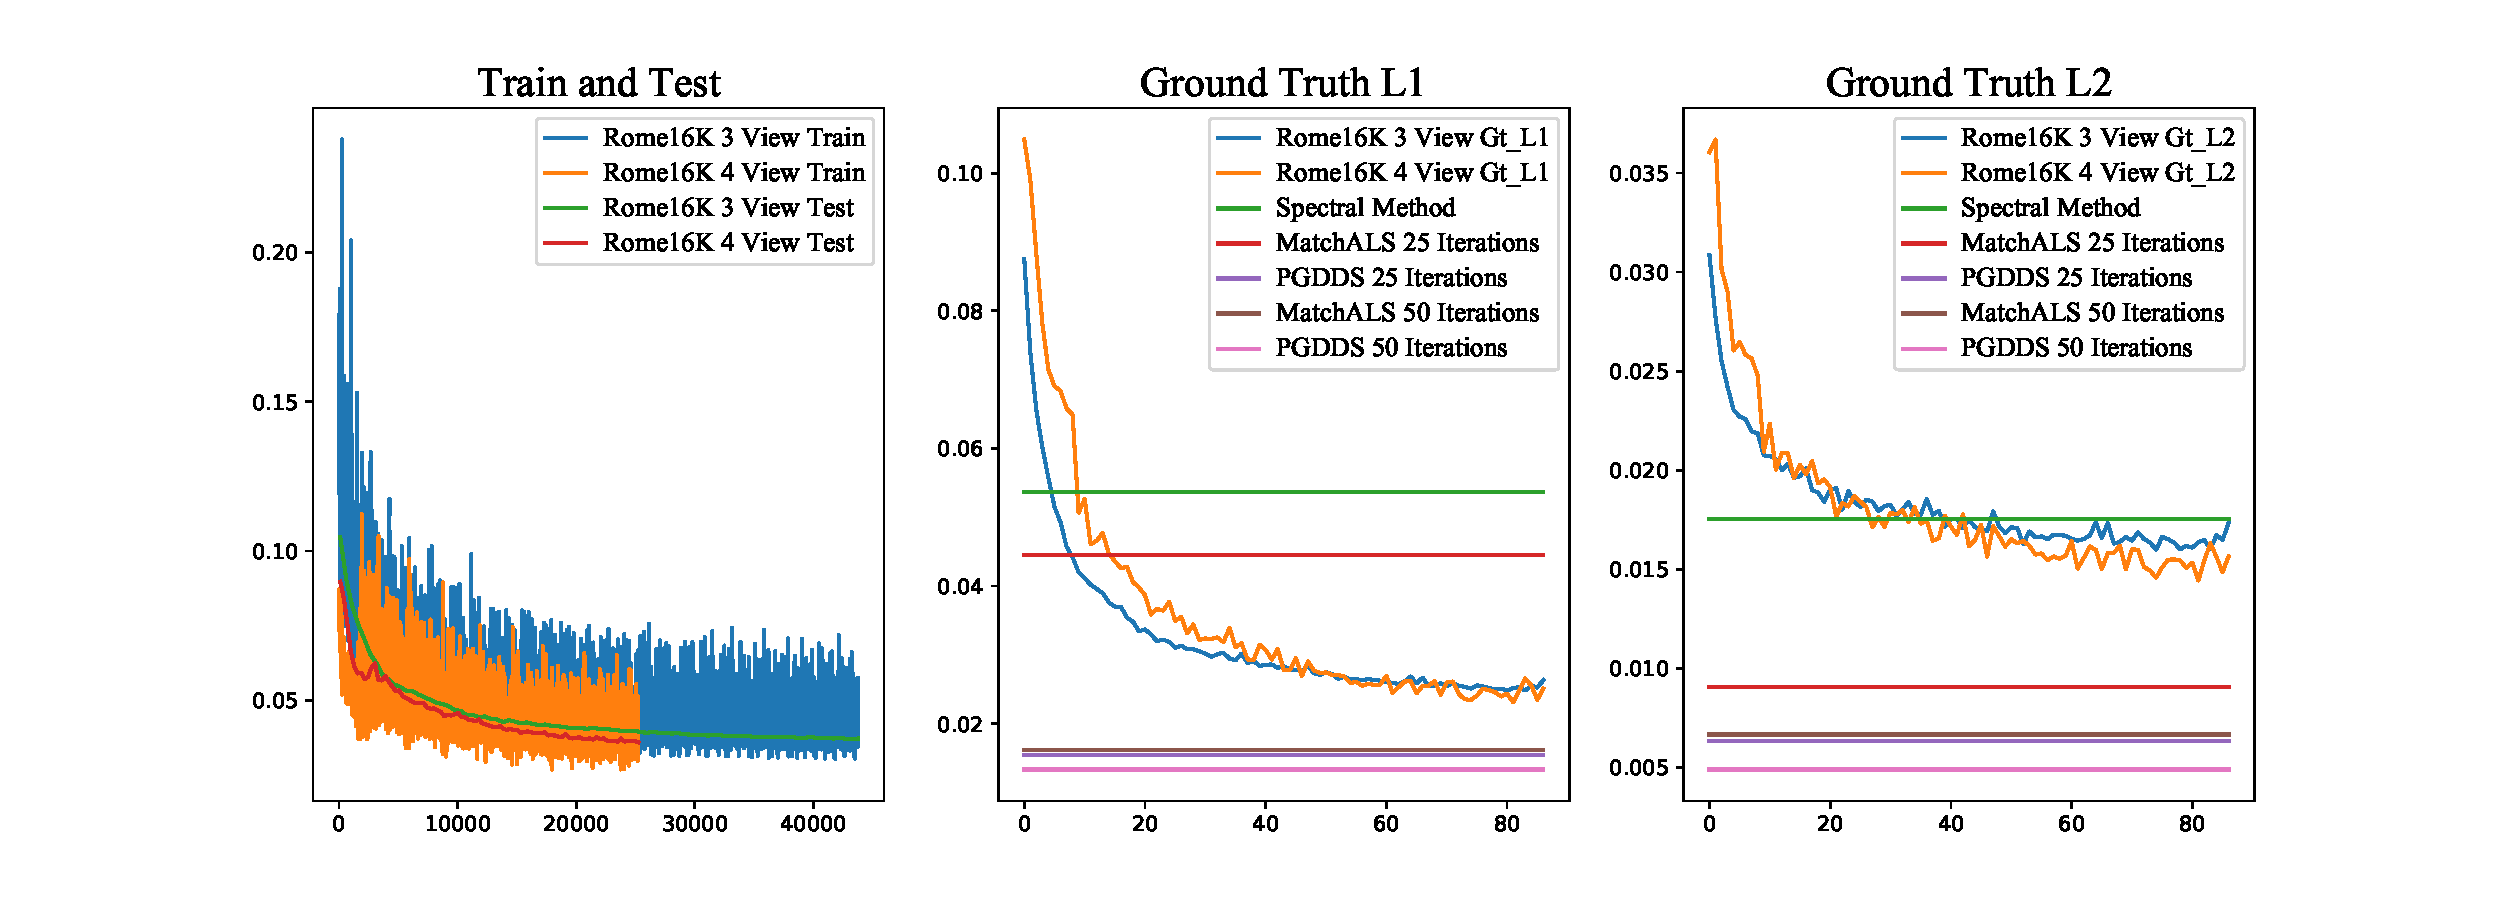
\includegraphics[width=0.8\linewidth]{figures/TrainingCurves.pdf}
  \end{center}
    \caption{
      Training curves with and without Geometric Training loss.
      The geometric training loss improves testing performance.
      Shown as horizontal lines are the state of the art optimization based baselines.
      Even with a simple network we compare well with them.
    }
  \label{fig:short}
\end{figure*}


\begin{figure*}
\begin{center}
  % \fbox{\rule{0pt}{2in} \rule{.9\linewidth}{0pt}}
  \includegraphics[width=0.8\linewidth]{figures/ExampleOutput.pdf}
  \end{center}
     \caption{Example output of our network. (a) Similarity Matrix of the of the embeddings (b) Histogram of feature similarities for pairs which correspond to the same 3D point, comparing our output features with the original SIFT features (c) Histogram of feature similarities for pairs which correspond to different 3D points, comparing our output features with the original SIFT features}
  \label{fig:short}
\end{figure*}
\subsection{Synthetic Graph Dataset}
We first test our method on synthetically generated data as a simple proof of concept.
To generate the data, we generate $p$ points, each with its own randomly generated descriptor.
To create the graph, we generate random permutation matrices, with a noise applied to it after generated.
The initial descriptors we use as input we created using the true descriptor plus some added Gaussian noise.
No geometric losses were added during training for these experiments.
However, the method was robust in testing with different noise functions and parameters.
The normalized noisy input descriptors are our baseline - they correlate with the true values but do not perserve the structure well.
However, with the GNN we are able to recover the true structure very well, as shown in \ref{fig:synthtable}.
All experiments were run with a 12 layer GCN with the ReLU nonlinearity and skip connections.
All were trained with the Adam optimizer \cite{kingma2014adam} and a learning rate $10^{-4}$


\subsection{Rome 16K Graph Dataset}
We  use the Rome16K dataset \cite{li2010location} to test our algorithm in real world settings.
Rome16K consistes of 16 thousand images of various historical sites in Rome extracted from Flickr, along with the 3D structure of the sites provided by bundle adjustment.
While not a standard dataset to test cycle consistency, other datasets had insufficient data to train a network on.
Rome16K is typically used to test bundle adjustment methods.
Therefore, to use for our method, we extract image triplets and quadtruplets with overlap of 80 points or more to test our algorithm on, with the points established as corresponding in the given bundle adjument output.
For the initial embedding we use the original 128 dimensional SIFT descriptors, normalized to have unit $L_2$ norm, the calibrated x-y position, the orientation, and log scale of the SIFT feature.
% For the outlier datasets, we take 79 correspondences and 1 non-corresponding point in each image.

For these experiments we train with the $L1$ norm and geometric consistency losses.
We evaluate on a test set using the ground truth adjacency matrix which we compute from the bundle adjustment given by the Rome16K dataset.
Traditional methods of evaluation use Precision and Recall, after making the labels 0 or 1.
We forgo this as our method was trained to output soft labels - we in turn make the labels soft for the optimization based methods.
For this method to work, we need the dimension of the embedding to be at least the number of unique points in the scene.
Picking the correct number is difficult a-priori, and is a problem with all cycle consistency based methods.
Here we use the ground truth dimension of the embedding to test both our method and the baselines.
For implementation details, our network has 12 layers, and was trained with the Adam optimizer \cite{kingma2014adam} with a learning rate of $10^{-4}$, with an exponentially decaying learning rate. We incorporate skip connections between the input, $6^{th}$, and $12^{th}$ layers, which greatly improved training convergence and testing performance (see supplemental material). 

We compare our method to spectral and optimization based baselines with different maximum iteration cutoffs. Our method is siginificatnly better than a simple spectral based optimization. Furthermore, our network, which only has 12 layers has the accuracy of the optimization based method MatchALS \cite{zhou2015multi} between 25 and 50 iterations. This inidicates that our method learns a more efficient update with each layer compared with an iteration in the optimization based methods.

%------------------------------------------------------------------------
\section{Conclusion}

We have shown a novel method for training feature matching.
This method can be employed even when labelled training data is not available, but can still incorporate geometric consistency into its losses.
We have demonstrated its effectiveness using experiments on the Rome16K dataset compared to the traditional optimization based baselines.
For future work we will investigate using more robust losses for outlier rejection and using higher order geometric constraints, such as the trifocal tensor, as additional loss terms.
A long term goal is to incorporate learning image level features into this pipeline
Moreover we hope to make this method distributed - with group norm, we cannot distribute in its current form.

{\small
\bibliographystyle{ieee}
\bibliography{mybib}
}

\end{document}
